\usepackage{siunitx}
\usepackage{pgfplots}
\usepackage{pgfplotstable}

\title{Example: Linear Regression with pgfplots}

\begin{document}

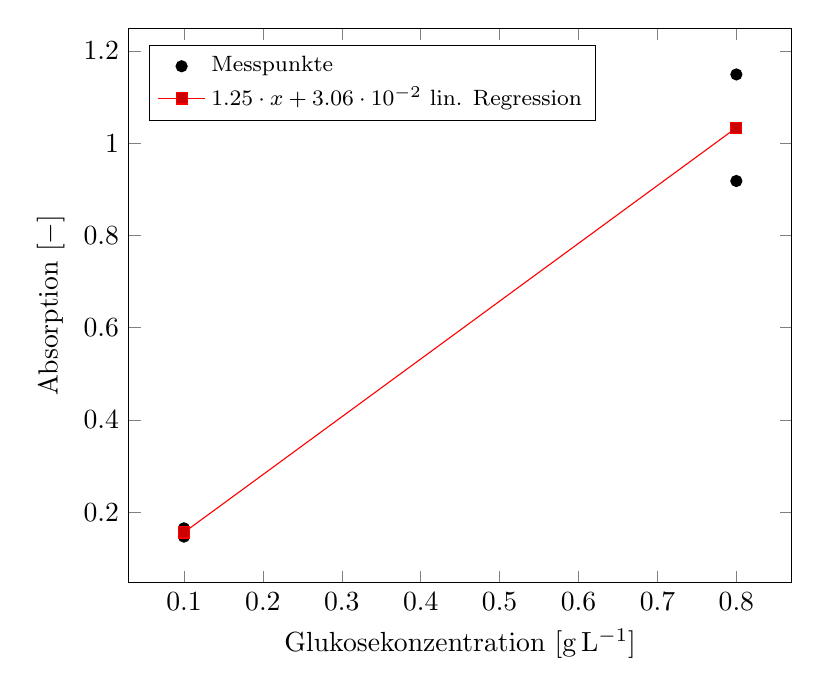
\begin{tikzpicture}
    \pgfplotsset{width=10cm,
        compat=1.3,
        legend style={font=\footnotesize}}
    \begin{axis}[
    xlabel={Glukosekonzentration [\si{\gram\per\liter}]},
    ylabel={Absorption $[-]$},
    legend cell align=left,
    legend pos=north west]
    \addplot[only marks] table[row sep=\\]{
        X Y\\
        0.1 0.147\\
        0.1 0.165\\
        0.8 0.918\\
        0.8 1.149\\
    };
    \addlegendentry{Messpunkte}
    \addplot table[row sep=\\,
    y={create col/linear regression={y=Y}}] % compute a linear regression from the
    %input table
    {
        X Y\\
        0.1 0.147\\
        0.1 0.165\\
        0.8 0.918\\
        0.8 1.149\\
    };
    \addlegendentry{%
        $\pgfmathprintnumber{\pgfplotstableregressiona} \cdot x
        \pgfmathprintnumber[print sign]{\pgfplotstableregressionb}$ lin. Regression} %
    \end{axis}
\end{tikzpicture}
    
\end{document}